\documentclass[11pt]{article}
\usepackage[margin=1in]{geometry}
\usepackage[T1]{fontenc}
\usepackage{lmodern}
\usepackage{amsmath}
\usepackage{booktabs}
\usepackage{graphicx}
\usepackage{caption}
\usepackage[numbers]{natbib}
\usepackage[hidelinks]{hyperref}
\newcommand{\RowsIn}{74,803}
\newcommand{\RowsOut}{70,225}
\newcommand{\AggRows}{4,355}
\newcommand{\OverlapRows}{223}
\newcommand{\Crops}{98}
\newcommand{\TestN}{17,896}
\newcommand{\ShockRate}{10.0}
\newcommand{\FixedCov}{0.751}
\newcommand{\RawFixedCov}{0.746}
\newcommand{\RollCov}{0.839}
\newcommand{\ReweightAge}{0.723}
\newcommand{\ReweightProv}{0.737}
\newcommand{\MonRollCov}{0.849}


\title{When 90\% Means 75\%: Conformal Crop Yield Intervals for Pakistan's Districts under Temporal Shift}
\author{Muzammal Hussain\\
Masmatix Innovations, Glasgow, United Kingdom\\
ORCID: \href{https://orcid.org/0009-0001-2570-5686}{0009-0001-2570-5686}}
\date{November 2026}

\begin{document}
\maketitle

\begin{abstract}
Year-ahead yield forecasts for districts and crops can support food-security planning, but only if their stated uncertainty can be trusted. We study split-conformal prediction intervals for one-year-ahead district-crop yields in Pakistan, using official district crop statistics from 1981--82 to 2024--25 (\RowsOut{} district-crop-year rows, \Crops{} crops, after cleaning). With a leakage-safe temporal design (training up to 2015--16, calibration on 2016--17 to 2019--20, test on 2020--21 to 2024--25), a pooled ridge model has a lower RMSE than persistence and a three-year median, but its nominal 90\% intervals cover only \FixedCov{} of \TestN{} test yields. The shortfall is present from the first test year, is concentrated in Punjab (0.600) and Balochistan (0.658), and is not caused by shifts in province proportions or in how many years of history each series has: reweighting the test results to the calibration-period mix still gives 0.737 and 0.723. Recalibrating each year on the previous four years raises coverage to \RollCov{} but nearly doubles interval width; an adaptive conformal update reaches 0.884 only with intervals too wide to use in some years. In an exploratory follow-up, province-wise rolling calibration reaches \MonRollCov{} with narrower intervals than pooled rolling calibration. No method reached the nominal level at a usable width. We release code, cleaning rules, a pre-specified protocol and all results.
\end{abstract}

\section{Introduction}
Pakistan's agriculture is exposed to heat, water shortages and floods; the 2022 monsoon floods alone caused damages and losses estimated at over USD 30 billion \citep{undp2022}. District-level yield forecasts are a natural input to early warning, and an interval forecast, a range that should contain the outcome with a stated probability, is more useful for planning than a single number.

Split-conformal prediction \citep{vovk2005,lei2018} gives such intervals with a finite-sample coverage guarantee, provided that calibration and test data are exchangeable. Yearly agricultural statistics are not: weather, reporting and crop mix change over time. Methods for conformal prediction under shift exist, including weighted schemes \citep{barber2023} and adaptive updates of the miscoverage level \citep{gibbs2021}, but there is little evidence on how much the guarantee fails, and how well simple fixes work, on real district-level crop data from a lower-middle-income country.

We ask: \emph{when a split-conformal interval is calibrated on 2016--2019 and used for 2020--2024, how far does its coverage fall, where does it fall, and does recalibration using only earlier years restore it?} Our contributions are:
\begin{enumerate}
  \item A leakage-safe benchmark on Pakistan Bureau of Statistics (PBS) district crop statistics, with documented cleaning, provenance hashes and a protocol committed before the main shift analysis was run.
  \item Evidence that nominal 90\% intervals cover about 75\% in 2020--2024, with the failure concentrated in two provinces and present across all series lengths.
  \item A comparison of five recalibration methods and an exploratory province-wise variant, showing a clear trade-off between coverage and width.
\end{enumerate}

\section{Data}
The source is the PBS district crop statistics in the machine-readable extract distributed by Data Darbar (file \texttt{crops\_district\_fy.parquet}, retrieved 10 November 2026, SHA-256 recorded in the repository). Each row is a district, crop and fiscal year with area, production and yield. Rows with missing values or unlabelled crops are dropped and never filled with zero, leaving \RowsIn{} rows for 122 districts.

Cleaning removes six aggregate labels (``Fodders Total'' and five ``Other \dots'' categories; \AggRows{} rows) and merges one pair of crop labels that differ only by case (``Potato'' and ``potato''), keeping the identifier with more rows and dropping \OverlapRows{} rows where both report the same district and year. The cleaned panel has \RowsOut{} rows and \Crops{} crops. All results are also reported without cleaning; fixed-interval coverage is \RawFixedCov{} without and \FixedCov{} with cleaning.

\section{Method}
\paragraph{Forecasting.} For target fiscal year $t$, features use only years before $t$: the last two log yields, the median of the last three, last-year log area and area growth, the province-crop median, a year trend and the gaps to the last two observations. A district-crop enters once it has three earlier observations. We compare persistence (last year's yield), the median of the last three yields, and one ridge regression pooled over all crops, all on the log-yield scale.

\paragraph{Intervals.} With absolute residuals $r_i = |y_i - \hat y_i|$ on a calibration set of size $n$, the split-conformal radius is the $\lceil (n+1)(1-\alpha) \rceil$-th smallest residual, and the interval is $\hat y \pm$ radius, with $\alpha = 0.1$. On the log scale a width $w$ means the interval spans a factor of $e^{w/2}$ above and below the forecast.

\paragraph{Recalibration methods.} All use only data observed before the target year. \emph{Fixed}: model trained on $\le$ 2015--16, radius from 2016--2019. \emph{Rolling}: same model, radius from the four years before $t$. \emph{Expanding}: radius from 2016 up to $t-1$. \emph{Refit + rolling}: ridge retrained on years $\le t-5$, radius from $t-4$ to $t-1$. \emph{ACI}: fixed calibration with the level updated once a year, $\alpha_{t+1} = \alpha_t + \gamma(\alpha - \mathrm{miss}_t)$, following \citet{gibbs2021}, with $\gamma \in \{0.1, 0.5\}$ fixed in advance and both reported.

\paragraph{Evaluation.} Coverage is the share of test yields inside their interval; 95\% confidence intervals use a bootstrap over district-crop series (500 replicates), so all years of one series are resampled together. These methods and metrics were committed to the repository before the real-data shift run. The province-wise (Mondrian, \citealp{vovk2005}) variant and the composition analysis in Section~\ref{sec:diag} were added after seeing those results and are exploratory.

\section{Results}
\paragraph{Point forecasts.} Table~\ref{tab:forecast} shows that ridge has the lowest RMSE, while persistence has the lowest MAE: ridge mainly reduces large errors. The test shock rate, a yield at least 15\% below the previous three-year median, is \ShockRate\%.

\begin{table}[h]
\centering
\caption{Point forecasts on the log-yield scale, test years 2020--21 to 2024--25 (\TestN{} forecasts, cleaned panel).}
\label{tab:forecast}
\begin{tabular}{lrr}
\toprule
Forecaster & RMSE & MAE \\
\midrule
Persistence (last year) & 0.464 & 0.198 \\
Median of last 3 years & 0.446 & 0.213 \\
Pooled ridge & 0.412 & 0.206 \\
\bottomrule
\end{tabular}

\end{table}

\paragraph{Coverage.} The fixed interval covers \FixedCov{} of test yields against a nominal 0.90 (Table~\ref{tab:coverage}). Every recalibration method raises coverage, but none reaches 0.90 at a usable width. Rolling calibration reaches \RollCov{} and nearly doubles the width (0.477 to 0.862, a factor of about 1.54 either side of the forecast instead of 1.27). Retraining the model as well adds nothing over rolling calibration alone. ACI with $\gamma = 0.5$ reaches 0.884 overall, but it oscillates: after a poor year its level falls close to zero and the interval becomes very wide (Table~\ref{tab:year}).

\begin{table}[h]
\centering
\caption{Test coverage of nominal 90\% intervals, 2020--21 to 2024--25. Width is the mean interval width on the log scale. The last two rows were added after the main results.}
\label{tab:coverage}
\begin{tabular}{lccc}
\toprule
Method & Coverage & 95\% CI & Mean width \\
\midrule
Fixed (2016--19) & 0.751 & 0.741--0.760 & 0.477 \\
Rolling, 4 years & 0.839 & 0.831--0.845 & 0.862 \\
Expanding & 0.814 & 0.806--0.821 & 0.692 \\
Refit + rolling, 4 years & 0.837 & 0.830--0.843 & 0.851 \\
ACI, $\gamma=0.1$ & 0.801 & 0.794--0.808 & 0.646 \\
ACI, $\gamma=0.5$ & 0.884 & 0.879--0.889 & 1.790 \\
\midrule
\multicolumn{4}{l}{\emph{Exploratory, added after the results above}} \\
By province, fixed & 0.757 & 0.749--0.766 & 0.478 \\
By province, rolling 4 years & 0.849 & 0.842--0.855 & 0.788 \\
\bottomrule
\end{tabular}

\end{table}

\begin{table}[h]
\centering
\small
\caption{Coverage by target year, with interval widths in two years.}
\label{tab:year}
\resizebox{\textwidth}{!}{\begin{tabular}{lcccccc}
\toprule
Target year & Fixed (2016--19) & Rolling, 4 years & Expanding & Refit + rolling, 4 years & ACI, $\gamma=0.1$ & ACI, $\gamma=0.5$ \\
\midrule
2020--21 & 0.718 & 0.718 & 0.718 & 0.718 & 0.718 & 0.718 \\
2021--22 & 0.735 & 0.802 & 0.785 & 0.802 & 0.763 & 0.988 \\
2022--23 & 0.711 & 0.817 & 0.785 & 0.814 & 0.765 & 0.798 \\
2023--24 & 0.751 & 0.898 & 0.857 & 0.895 & 0.843 & 0.993 \\
2024--25 & 0.836 & 0.944 & 0.913 & 0.942 & 0.908 & 0.908 \\
\midrule
Width 2021--22 & 0.48 & 0.67 & 0.61 & 0.67 & 0.55 & 2.23 \\
Width 2023--24 & 0.48 & 1.08 & 0.80 & 1.06 & 0.75 & 4.56 \\
\bottomrule
\end{tabular}
}
\end{table}

\begin{figure}[h]
\centering
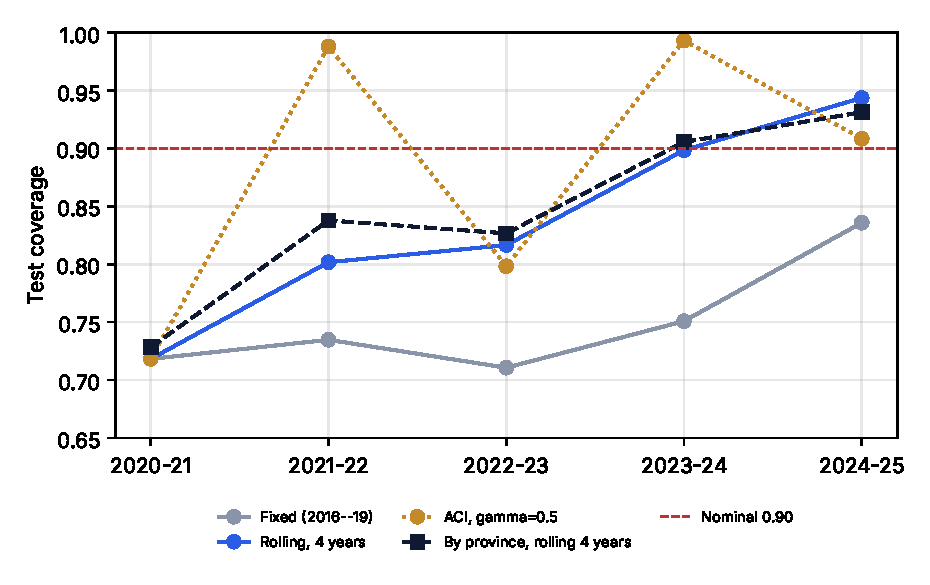
\includegraphics[width=0.75\textwidth]{figures/coverage_by_year.pdf}
\caption{Coverage by target year for selected methods. The dashed line is the nominal 0.90.}
\label{fig:year}
\end{figure}

\section{Where the guarantee fails}\label{sec:diag}
Coverage is already 0.718 in 2020--21, the first test year, so the failure does not start with the 2022 floods. Table~\ref{tab:comp} compares the calibration and test sets. The mix did change: Punjab's share fell from 0.419 to 0.347, and the largest group of test forecasts (48\%) comes from series with 11--20 years of history, against 2\% in calibration. But coverage fell sharply within Punjab (0.885 to 0.600) and Balochistan (0.906 to 0.658), and within every series-length group, while Sindh (0.950) and Khyber Pakhtunkhwa (0.900) stayed at or above the nominal level. Holding the calibration-period shares fixed and using test-period coverage within groups gives \ReweightProv{} by province and \ReweightAge{} by series length, so the change in mix explains little of the gap.

\begin{table}[h]
\centering
\caption{Calibration and test sets: share of forecasts and fixed-interval coverage within each group.}
\label{tab:comp}
\begin{tabular}{lcccc}
\toprule
 & \multicolumn{2}{c}{Calibration 2016--19} & \multicolumn{2}{c}{Test 2020--24} \\
 & Share & Coverage & Share & Coverage \\
\midrule
\emph{Province} \\
\quad Balochistan & 0.188 & 0.906 & 0.228 & 0.658 \\
\quad Islamabad Capital Territory & 0.006 & 0.880 & 0.001 & 0.762 \\
\quad Khyber Pakhtunkhwa & 0.203 & 0.869 & 0.221 & 0.900 \\
\quad Punjab & 0.419 & 0.885 & 0.347 & 0.600 \\
\quad Sindh & 0.185 & 0.963 & 0.204 & 0.950 \\
\emph{Years of history} \\
\quad 3--5 & 0.224 & 0.884 & 0.045 & 0.639 \\
\quad 6--10 & 0.679 & 0.904 & 0.391 & 0.734 \\
\quad 11--20 & 0.023 & 0.912 & 0.480 & 0.755 \\
\quad 21+ & 0.075 & 0.906 & 0.083 & 0.867 \\
\bottomrule
\end{tabular}

\end{table}

Because the failure is province-specific, we tried province-wise radii (Table~\ref{tab:prov}). With fixed calibration this changes little (0.757), since Punjab's and Balochistan's calibration residuals were not unusually large. Combined with rolling calibration it reaches \MonRollCov{} with a mean width of 0.788, narrower than pooled rolling calibration (0.862), because Sindh and Khyber Pakhtunkhwa receive narrow intervals and Punjab and Balochistan wide ones. Punjab still reaches only 0.791.

\begin{table}[h]
\centering
\small
\caption{Coverage (mean width) by province. Islamabad has fewer than 50 calibration residuals and uses the pooled radius.}
\label{tab:prov}
\resizebox{\textwidth}{!}{\begin{tabular}{lrccc}
\toprule
Province & $n$ & Pooled, fixed & Pooled, rolling 4 years & By province, rolling 4 years \\
\midrule
Balochistan & 4075 & 0.658 (0.48) & 0.749 (0.87) & 0.815 (1.16) \\
Islamabad Capital Territory & 21 & 0.762 (0.48) & 0.809 (0.69) & 0.809 (0.67) \\
Khyber Pakhtunkhwa & 3951 & 0.900 (0.48) & 0.939 (0.86) & 0.926 (0.59) \\
Punjab & 6205 & 0.600 (0.48) & 0.757 (0.85) & 0.791 (0.99) \\
Sindh & 3644 & 0.950 (0.48) & 0.969 (0.86) & 0.900 (0.25) \\
\bottomrule
\end{tabular}
}
\end{table}

\section{Discussion and limitations}
For users of district crop forecasts in Pakistan, the main message is that a ``90\%'' interval calibrated on recent years can hold about three times in four, and much less in Punjab and Balochistan. Recalibrating every year on recent data, separately by province, is a cheap improvement and is what we would recommend over a fixed calibration, but it still under-covers.

We did not test why Punjab and Balochistan changed. Two candidate explanations are worth testing. First, crop mix may have changed within districts, for example a move away from cotton in parts of South Punjab; this can be checked directly in the area columns of the panel. Second, irrigation has changed: Reuters reported in 2025 that around 650,000 tube wells in Pakistan run on solar power, and that the share of Punjab where the water table is below the critical 60 feet rose by about a quarter between 2020 and 2024 \citep{reuters2025}. Either could change yield variability in ways that a model and calibration fitted on earlier years do not capture.

This study has limits. District yields are administrative estimates, and district boundaries and codes changed over four decades; some areas are missing from the extract. One pooled linear model covers very different crops, and no weather or satellite data are used, so better models may shrink the problem. Only five test years are available, and the province-wise analysis was added after seeing the results, so it needs confirmation on later years. Coverage is marginal over the test set; it does not guarantee coverage for any single crop or district. We do not identify causes of the shift, and our results are not official PBS estimates.

\section{Reproducibility}
Code, cleaning rules, the protocol and all result files are at \url{https://github.com/MHKhan50/harvestguard-pk}. Release v0.3.1 is archived on Zenodo, \href{https://doi.org/10.5281/zenodo.24138382}{doi:10.5281/zenodo.24138382}. The tables in this paper are generated from the committed result files by \texttt{paper/make\_tables.py}.

\bibliographystyle{plainnat}
\bibliography{references}
\end{document}
